\question{
    The pentagonal numbers are the integers that count the
number of ``coins" that can be arranged to form pentagons.
Some examples are shown below.

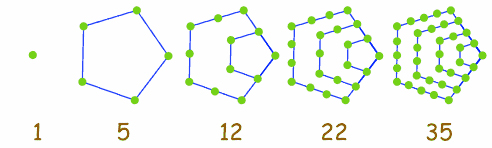
\includegraphics[width=4in]{images/pentagonal-numbers.jpg}
}


\begin{parts}
    \part{
        Determine a recursion equation for the pentagonal
        numbers and explain how this can be understood
        from the geometry.  For example, we could see that
        in the triangular numbers that we were simply
        adding a new row with
        $n$ numbers to see that $t_n=t_{n-1}+n$.
    }
    \begin{solution}
        Each time we add 3 sides with $n$ points each
        and subtract 2 points.
        So, the $n^{th}$ pentagonal number
        $p_n$ is given by
        $$p_{n}=p_{n-1} + 3n -2$$
        where the base case is given by $p_1=1$.
    \end{solution}

    \part{
        Use the recursion equation in the previous
        part to write the equation as a sum.

        For example, we saw that $t_n=t_{n-1}+n$
        and then that $t_n=\sum_{i=1}^{n} i$.
        
        We also showed that the square numbers
        $s_n=s_{n-1}+2n-1$ and then that
        $s_n=\sum_{i=1}^n(2i-1).$
    }
    \begin{solution}
        Using the recursive
        definition, the $nth$ term is given by:
        $$p_n = \sum_{i=1}^n{3i-2}$$
        \begin{note}
            $p_n = s_n+t_{n-1}$,
            where $t_n$ is the $nth$ triangular
        number and $s_n$ is the $nth$ square
        number.
        \end{note}
    
    \end{solution}

    \part{
        Determine a closed-form solution for the pentagonal
        numbers.  Use induction to show that this is
        equivalent to the recursion equation stated above.
        For example, we showed that
        $\sum_{i=1}^n i=1+2+\ldots +n=\frac{n(n+1)}{2}$
        using induction in class.
    }
    \begin{solution}
        Let, 
        \begin{equation}
            H_k: p_k = \frac{k(3k-1)}{2}.
        \end{equation}

        Here, we see that the base case $p_1=2/2=1$, which
        is true. Assuming that the statement $H_k$ is true
        for some integer $k>1$, we 
        have
        \begin{align*}
            p_{k+1} &= p_k+3(k+1)-2\\
            &=\frac{k(3k-1)}{2} +3k+1\\
            &=\frac{3k^2-k+6k+2}{2}\\
            &=\frac{3k^2-5k+2}{2}\\
            &=\frac{(k+1)(3(k+1)-1)}{2}
        \end{align*}
        Then, since $H_k\implies H_{k+1}$, the statement is
        true for all integers $k\ge 0$.
    \end{solution}
\end{parts}